% THIS IS SIGPROC-SP.TEX - VERSION 3.1
% WORKS WITH V3.2SP OF ACM_PROC_ARTICLE-SP.CLS
% APRIL 2009
%
% It is an example file showing how to use the 'acm_proc_article-sp.cls' V3.2SP
% LaTeX2e document class file for Conference Proceedings submissions.
% ----------------------------------------------------------------------------------------------------------------
% This .tex file (and associated .cls V3.2SP) *DOES NOT* produce:
%       1) The Permission Statement
%       2) The Conference (location) Info information
%       3) The Copyright Line with ACM data
%       4) Page numbering
% ---------------------------------------------------------------------------------------------------------------
% It is an example which *does* use the .bib file (from which the .bbl file
% is produced).
% REMEMBER HOWEVER: After having produced the .bbl file,
% and prior to final submission,
% you need to 'insert'  your .bbl file into your source .tex file so as to provide
% ONE 'self-contained' source file.
%
% Questions regarding SIGS should be sent to
% Adrienne Griscti ---> griscti@acm.org
%
% Questions/suggestions regarding the guidelines, .tex and .cls files, etc. to
% Gerald Murray ---> murray@hq.acm.org
%
% For tracking purposes - this is V3.1SP - APRIL 2009

\documentclass{acm_proc_article-sp}

\usepackage[colorlinks=true,linkcolor=blue]{hyperref}	% For hyper links
\usepackage{caption}
\usepackage{subcaption}
\usepackage{bbm}

\usepackage{CJKutf8} 
\usepackage{ucs} 
\usepackage[encapsulated]{CJK} 
\newcommand{\myfont}{gbsn}

%\usepackage{fontspec} 
%\usepackage{xeCJK}
%\setCJKmainfont{BiauKai}

%\usepackage{polyglossia}
%\setmainlanguage{english}
%\setotherlanguage{arabic}
%\newfontfamily\arabicfont{Scheherazade}

\graphicspath{ {./Figures/} }

\begin{document}

\title{Bootstrapping Language-Agnostic Event Detection in Social Media Streams with Sporting Events}
%
% You need the command \numberofauthors to handle the 'placement
% and alignment' of the authors beneath the title.
%
% For aesthetic reasons, we recommend 'three authors at a time'
% i.e. three 'name/affiliation blocks' be placed beneath the title.
%
% NOTE: You are NOT restricted in how many 'rows' of
% "name/affiliations" may appear. We just ask that you restrict
% the number of 'columns' to three.
%
% Because of the available 'opening page real-estate'
% we ask you to refrain from putting more than six authors
% (two rows with three columns) beneath the article title.
% More than six makes the first-page appear very cluttered indeed.
%
% Use the \alignauthor commands to handle the names
% and affiliations for an 'aesthetic maximum' of six authors.
% Add names, affiliations, addresses for
% the seventh etc. author(s) as the argument for the
% \additionalauthors command.
% These 'additional authors' will be output/set for you
% without further effort on your part as the last section in
% the body of your article BEFORE References or any Appendices.

\numberofauthors{3} %  in this sample file, there are a *total*
% of EIGHT authors. SIX appear on the 'first-page' (for formatting
% reasons) and the remaining two appear in the \additionalauthors section.
%
\author{
% You can go ahead and credit any number of authors here,
% e.g. one 'row of three' or two rows (consisting of one row of three
% and a second row of one, two or three).
%
% The command \alignauthor (no curly braces needed) should
% precede each author name, affiliation/snail-mail address and
% e-mail address. Additionally, tag each line of
% affiliation/address with \affaddr, and tag the
% e-mail address with \email.
%
% 1st. author
\alignauthor
Cody Buntain\\
       \affaddr{Dept. of Computer Science}\\
       \affaddr{University of Maryland}\\
       \affaddr{College Park, Maryland 20742}\\
       \email{cbuntain@cs.umd.edu}
% 2nd. author
\alignauthor
Jimmy Lin\\
       \affaddr{College of Information Studies}\\
       \affaddr{University of Maryland}\\
       \affaddr{College Park, Maryland 20742}\\
       \email{jimmylin@cs.umd.edu}
\alignauthor
Jen Golbeck\\
       \affaddr{College of Information Studies}\\
       \affaddr{University of Maryland}\\
       \affaddr{College Park, Maryland 20742}\\
       \email{golbeck@cs.umd.edu}
% Just remember to make sure that the TOTAL number of authors
% is the number that will appear on the first page PLUS the
% number that will appear in the \additionalauthors section.
}

\maketitle
\begin{abstract}
{\color{red}
Lorem ipsum dolor sit amet, consectetur adipiscing elit. Etiam tristique quam dolor, sed fermentum eros commodo eget. Nunc sem ante, tempor gravida gravida quis, vehicula nec dui. Integer hendrerit laoreet mi eu commodo. Integer lacus metus, suscipit at dignissim eget, blandit eget velit. Aenean ac porta metus, ac ultrices sem. Integer tincidunt arcu tortor, id sollicitudin lorem finibus nec. Morbi dignissim purus eget est porta interdum. Nulla faucibus lacinia dignissim. Praesent at nibh dignissim, placerat arcu sit amet, interdum orci.

In volutpat gravida turpis, nec ornare quam. Nam elementum elit non risus rhoncus, facilisis feugiat massa commodo. Vestibulum tempor felis et porttitor vestibulum. Nullam odio neque, ornare in interdum vel, volutpat quis ipsum. Integer vel finibus erat. Quisque eu mi vehicula erat imperdiet vestibulum. Sed laoreet eros lacinia aliquam mollis. Donec fringilla ante id ex pellentesque ultrices. Interdum et malesuada fames ac ante ipsum primis in faucibus.
}
\end{abstract}

% A category with the (minimum) three required fields
\category{H.2.8}{Database Applications}{Data Mining}
\category{\\H.3.3}{Information Search and Retrieval}{Information Filtering}

\keywords{event detection, twitter, social networks, temporal features}

%\keywords{ACM proceedings, \LaTeX, text tagging} % NOT required for Proceedings

\section{Introduction}

Social media's ubiquity has drastically altered the velocity with which we spread and consume information, transforming how news and opinions propagate across the planet. 
This democratization of information dissemination has both researchers and traditional media organizations considering social media as a viable complement and/or alternative to real-time news sources.
For instance, existing research demonstrates social media can perform on par with existing newswire sources for certain types of breaking stories \cite{petrovic2013can}.
While such social media-based systems are able to detect noteworthy events rapidly and in near real time, they often come with restrictive assumptions to facilitate the event-detection task.
These assumptions might be requiring pre-specified classes of interesting event, limiting target languages, setting event-centric queries, and preprocessing/filtering data through expensive language models.
Resulting systems are brittle and inflexible in application and are difficult to adapt to new domains, languages, or events.
Forgoing these simplifying restrictions and processing an unfiltered social media stream is a more difficult task given the volume of noise in such sources, but advantages like multi-language event detection and unexpected event discovery have many practical and important applications currently  unsatisfied by existing technology.

Existing work already achieves acceptable performance in detecting events within social media streams when event types and keywords are known, but what if we could achieve the same level of performance in a language-agnostic way and without the need to specify keywords or filter the streams?
Given the ``unreasonable effectiveness of data'' and the shear volume of social media content  generated per minute (hundreds of thousands of comments, statuses, and photos on Facebook alone as of 2012 \cite{Pring2012}), it is possible that usage patterns alone could provide interesting cues for detecting events without relying on linguistic understanding and related drawbacks.
This paper pursues such an alternative avenue for unfiltered event detection by disregarding language semantics and focusing on the temporal patterns that comprise breaking news and high-impact events.

To explore these questions, we propose a set of features for learning patterns of increased token usage, or bursts, in the Twitter stream in response to key moments in large sporting competitions.
From these features, we then build an ensemble classifier to detect such bursting tokens from messages in the Twitter stream, called ``tweets.''
Then, using frequencies of these classified tokens, we demonstrate the feasibility of detecting new events of interest from unfiltered Twitter data.
To ground this exploration, we start by modeling large sporting competitions as such events are both highly followed and occur regularly but also include unpredictable patterns of sub-events around points scored, fouls committed, and other occurrences of high interest.
Experiments on several such sporting competitions illustrate how a language-agnostic, burst-centric technique performs in comparison to baseline keyword-centric methods while simultaneously providing additional insight across languages and without text normalization or filtering.
Finally, we apply the models learned in the sporting domain to earthquake detection and show performance commensurate with existing research.

% I hate these kinds of paragraphs
%Prior to presenting our work, however, we first establish the context and foundations upon which our research builds by briefly describing the relevant work in this area (Section \ref{sect:relatedWork}). 
%We follow up with descriptions of data collection and methods for comparing our technique to an existing token-centric baseline before providing details on our features for burst detection, the components of our ensemble classifier, and how the baseline operates (Section \ref{sect:methods}).
%Results from these experiments and their analyses are then presented (Sections \ref{sect:results} and \ref{sect:analysis} respectively) before we close with ideas for future work and conclusions.

\section{Related Work}
\label{sect:relatedWork}

Detecting events by leveraging digital media has fascinated researchers for nearly twenty years now, with new methods, breakthroughs, and technologies emerging every few years.
As a result, this subfield has experienced a series of evolutionary steps, each of which integrates the latest available techniques and data sources, starting from early digital newsprint to blogs and now to social media.
Early stages of this research started in the mid-nineties, however, with the Defense Advanced Research Projects Agency's (DARPA) Topic Detection and Tracking (TDT) initiative \cite{Allan98topicdetection}.
By the late nineties, DARPA's programs demonstrated feasibility in detecting new topics from traditional media sources, but as Allan, Papka, and Lavrenko discussed in 1998, the utility and limitations of these approaches required additional work to see real success \cite{allan1998line}.
Even in that early work, Allan et al. were already discussing the tradeoffs of using pre-defined keyword sets and event classes when detecting new events, an issue researchers have begun to address only recently.
It is also important to note that, at this nascent stage, topic detection and event detection were relatively synonymous in the literature.

Though this early research focused primarily on topic detection from newsprint and traditional media sources, Kleinberg's 2002 paper altered the TDT landscape by applying topic detection to non-traditional data sources like his personal email archive and by introducing what appears to be the first real treatment of burst analysis in ``document streams that arrive continuously over time'' rather than  static collections \cite{Kleinberg:2002:BHS:775047.775061}. 
Despite this introduction of the streaming context, Kleinberg's methods cast topic detection as a retrospective optimization problem in which each token was assigned a set of states describing its usage.
From this description, Kleinberg was able to leverage existing work on hidden Markov models (HMMs) to find optimal sequences of high usage states, or bursts, and low usage states from which he could detect events (and even construct arbitrarily complex burst states to develop event hierarchies).
Kleinberg's examination here laid much of the foundation for the focus on topic bursts that characterized much of the proceeding research in this area.

Following from Kleinberg's work and the increasing size of digital content creation on the Internet, several new approaches to topic detection emerged.
Notably, topic detection divided into two distinct tasks: identifying topics in data via algorithms like Latent Dirichlet Allocation (LDA) \cite{blei2003latent} and detecting events from text.
Since our research focuses on events rather than topics, early event detection work like that from Fung et al. in 2005 is especially interesting \cite{Fung:2005:PFB:1083592.1083616}.
Fung et al. extended Kleinberg's burst detection scheme by identifying bursty keywords from digital newspapers and clustering these keywords into groups to identify bursty events, which displayed success in identifying trending events in an English-language newspaper from Hong Kong.

Along with new interest in burst-centric research, another important trend starting around this time was the integration of additional data sources beyond traditional newsprint, most significant of which was the increased usage of blog content.
Blogs offered direct insight into the social consciousness in a way that was previously unavailable via traditional media since blogs include a great deal of social information regarding the author.
Zhao et al. took advantage of this additional social information in their 2007 work on flow-based event detection from 2007 \cite{Zhao2007}.
This work viewed blog dynamics and information flow within them as a graph problem in which nodes represent ``social actors'' and edges represent information exchanges between them.
By integrating this social data with the textual and temporal techniques described above, Zhao et al. were able to identify events with high accuracy in two social datasets: the Enron email dataset and the Dailykos dataset.
Similarly, Bansal's group from the University of Toronto developed the Blogscope project to identify trending and bursty keywords by location as well as time across the entire ``blogosphere'' \cite{Bansal:2007:BSO:1325851.1326028,Bansal:2007:BSA:1242572.1242802}.

\subsection{Event Detection in Microblogs}

Soon after the research community began experimenting with alternative media sources like blogs, microblogging platforms began their rise in popularity.
These microblogging platforms include websites like Twitter and Sina Weibo and are characterized by constrained post sizes and broadcast information dissemination (e.g., Twitter constrains user posts to 140 characters).
A great deal of research exists that explores how the data posted to these networks can be leveraged for social good projects like event detection.
It is worth noting the majority of this research makes use of data from Twitter's network, likely because Twitter data is relatively easy to acquire using Twitter's APIs.

One of the most well-known works in detecting events from microblogs is Sakaki, Okazaki, and Matsuo's 2010 paper on detecting earthquakes in Japan using Twitter \cite{Sakaki:2010:EST:1772690.1772777}.
In their paper, Sakaki et al. show that not only can one detect earthquakes on Twitter but also that it can be done simply by tracking frequencies of earthquake-related tokens, and surprisingly, doing so can outperform geological earthquake detection tools since digital data propagates faster than tremor waves in the Earth's crust.
Though this research is limited in that it requires pre-specified tokens and is highly domain- and location-specific (Japan has a high density of Twitter users, so earthquake detection may perform less well in areas with fewer Twitter users), it demonstrates a significant use case and the potential of such applications.

Along with the research of Sakaki et al., 2010 saw two other relevant papers: Lin et al.'s construction of a probabilistic popular event tracker (PET) \cite{Lin:2010:PSM:1835804.1835922} and Petrovi\'{c}, Osborne, and Lavrenko's application of locality-sensitive hashing (LSH) for detecting first-story tweets from Twitter streams \cite{Petrovic:2010:SFS:1857999.1858020}.
Lin's work is interesting for a number of reasons: first, it seems to be one of the first treatments to leverage probabilistic models to discriminate between common tokens and informational tokens by assigning them to either a background or topical language model, whereas other methods often relied on pre-specified lists of stop words.
Secondly, Lin's integration of social and structural features into the event detection task demonstrated that real performance enhancements can be gained through non-textual features.
Thirdly, their paper relates well to Kleinberg's initial work on bursty topic detection by illustrating how his state machine approach is a degenerate case of the PET model.
Like the majority of its contemporary systems, however, PET also requires seeding with a pre-specified list of tokens to guide its event detection.

Petrovi\'{c}'s research on clustering in Twitter avoids the need for seeding keywords by instead focusing on the practical considerations of clustering large streams of data quickly.
That is, rather than construct a probabilistic mixture model for each token, Petrovi\'{c} focuses on methods for clustering tweets that contain similar tokens into topical clusters.
While typical clustering algorithms require distance calculations for all pairwise messages, LSH facilitates rapid clustering at the scale necessary to support event detection in Twitter streams by restricting the number of tweets compared to only those within some threshold of similarity.
Once these clusters are generated, Petrovi\'{c} was able to track their growth over time to determine impact and find the ``first story'' or tweet for a given event.
This research was originally unique in that it was one of the early methods that did not require pre-specified seed tokens for detecting events and has been very influential in the field, resulting in a number of additional publications to demonstrate its utility in breaking news and for high-impact crisis events \cite{Petrovic:2012:UPI:2382029.2382072,osborne2014real,petrovic2013can,6601695}.
That being said, a key weakness in Petrovi\'{c}'s work is its reliance on semantic similarity between tweets, which limits its ability to operate in mixed-language environments.

Similar to Petrovi\'{c}, Weng and Lee's 2011 paper on EDCoW, short for Event Detection with Clustering of Wavelet-based Signals, is also able to identify events from Twitter without seed keywords \cite{weng2011event}.
After stringent filtering (removing stop words, common words, and non-English tokens), EDCoW uses wavelet analysis to isolate and identify bursts in token usage as a sliding window advances along the social media stream.
Highly significant bursts are then cast as a cross-correlation matrix against which a graph partitioning algorithm is run to construct topical clusters from bursty tokens.
Besides the heavy filtering of the input data, this approach exhibits notable similarities with the language-agnostic method described herein with its reliance on bursts to detect event-related tokens; the methods described in Weng and Lee's paper, however, operate in a more retrospective manner, focusing on the level of daily news rather than breaking event detection on which our research focuses.
Becker, Naaman, and Gravano's 2011 paper on identifying events in Twitter also fall under this label of retrospective analysis, but their findings also demonstrate reasonable performance in identifying events in Twitter by leveraging classification tasks to separate tweets into those on ``real-world events'' versus non-event messages \cite{becker2011beyond-tr,becker2011beyond}.
Similarly, Diao et al. also employ a retrospective technique to separate tweets into global, event-related topics and personal topics \cite{diao2012finding}.

Beyond these relatively general efforts, several domain-specific methods exist that target event detection in sporting events \cite{vasudevan2013twitter,Zhao2011,lanagan2011using}.
Lanagan and Smeaton's work, however, is of particular interest because it relies almost solely on analyzing the per-second volume of messages in Twitter \cite{lanagan2011using}.
Though relatively naive, this frequency-centric approach is able to detect large bursts on Twitter in high-impact events like the NFL's Super Bowl and can do so without reliance on complex linguist analysis.
Additionally, such a straightforward approach works very well in a streaming context as very little information must be kept in memory.
Unfortunately, two main disadvantages exist with this technique: first, detecting a burst would provide evidence of an event, but it would be difficult to gain insight into what that event actually is without additional processing.
Secondly, as described in their paper, a pure volumetric approach can be hampered by limitations on Twitter's public stream, which has an upper limit on the number of messages per minute one can capture.
The approach we describe below addresses both of these deficiencies.

Finally, the most recent work that shares the most in common with the our research is the 2013 paper by Xie et al. on TopicSketch \cite{xie2013topicsketch}.
Like us, TopicSketch's authors seek to perform real-time event detection from Twitter streams ``without pre-defined topical keywords'' by maintaining acceleration features across three levels of granularity: individual token, bigram, and total stream.
As with Petrovi\'{c}'s use of LSH, Xie et al. leverage ``sketches'' and dimensionality reduction to facilitate the event detection task and also relies on language-specific similarities, but Xie et al. also focus only on tweets from Singapore rather than the worldwide stream.
In contrast, our approach is differentiated primarily in its language-agnosticism and its use of the unfiltered stream from Twitter's global network.

\subsection{Twitter's Trending Topics}

Given our focus on Twitter and the data provided by their streaming sources, it is worth taking a moment to differentiate our techniques from Twitter's existing ``Trending Topics'' offering.
When a user visit's Twitter's website, she is immediately greeted with her personal feed as well as a listing of trending topics for her city, country, worldwide, or nearly any location she chooses.
These topics offer a great deal of insight into the current popular topics on Twitter, but the main differentiating factor we try to identify is that these popular topics are not necessarily connected to specific events that we target.
Rather, popular memetic content like ``\#MyLovelifeInMoveTitles'' often appear on the list of trending topics.
Additionally, Twitter monetizes these trending topics as a form of advertising \cite{Sydell2011}.  
These trending topics also can be more high-level than the point events that we seek to identify: for instance, during the World Cup, particular matches or the tournament in general were identified as trending topics by Twitter, but individual events like goals or penalty cards in those matches were not.
It should be clear then that Twitter's trending topics serves a different purpose than the streaming event detection described herein.

\section{Techniques for Streaming Event Detection}
\label{sect:methods}

This paper's primary goal is to demonstrate the feasibility of detecting significant events from social media streams without relying on pre-specified queries and instead by identifying temporal bursts in token usage and analyzing their frequencies (we refer to this language-agnostic, burst-centric technique as LABurst).
To this end, we compare LABurst's performance with that of a baseline token-based technique in detecting specific events within a variety of major sporting competitions.
Then, we show applications outside the sports domain by applying LABurst to the task of detecting earthquakes from social media soon after they occur.
This section's remainder defines these detection tasks, presents our experimental framework, details the data sources used, and outlines both the baseline technique and our LABurst method.

\subsection{Problem Definition}

Prior to any deep description on methods, we must first define an ``event'' and a ``burst'' within the context of this research.
Though the term ``event'' is vague and overridden in many contexts, we can borrow from existing works like Allan et al.'s preliminary report on event detection and tracking and Raimond and Abdallah's Event Ontology \cite{Raimond2007,allan1998line}.
From these sources, one could define an event as ``something that happens at a particular time and place'' and can be composed of one or more brief ``sub-events'' that occur within the context of the larger event.
For the purposes of this paper, however, we further restrict our definition to \emph{instantaneous} events and sub-events, or those events that occur at a specific place and time \emph{and} have a negligible amount of time between start and end.
Examples of such instantaneous events include a point scored in a game, a particular explosion during some terrorist attack, or a particular tremor in an earthquake.
These instantaneous events are interesting and harder to identify than their longer-term counterparts because one may not know tokens relevant to these brief events until the event is occurring, and by the time one can react, such a short-term event would already be over. 

Corresponding to these brief events, we define a burst in a token's usage as a sudden increase in the frequency with which that token appears in a data stream.
Like ``event,'' ``burst'' is also vague and can be applied at various levels of temporal granularity (seconds, minutes, hours, days, etc.).
As an example, ``Obama'' would have experienced a burst in usage over a period of months leading into the 2008 Democratic Presidential Primary as President Obama was relatively unknown prior to that. 
Tokens like ``earthquake'' or ``superbowl,'' on the other hand, would experience more drastic bursts in much shorter periods just around the time of a specific event.
We refer to such tokens as ``bursty.''
Again, for our purposes, we focus only on bursts that occur within a minute (or just a few minutes). 
It's worth noting here that bursts need not be symmetric; that is, a drastic uptick in frequency need not be followed by an equally dramatic dip in usage.

Now, if we let $E$ denote the set of all minutes $t$ in which an event occurs, then the indicator function $\mathbbm{1}_E(t)$ returns a $1$ for all times $t$ in which an event occurs, and $0$ for all other values of $t$. 
We can now define the event detection task as constructing a function that approximates this indicator function $\mathbbm{1}_E(t)$.
To account for possible lag in experiencing the event, typing out a message about the event, and the message actually posting to a social media server, we relax this task slightly by using the set $E'$ where, for all $t \in E$, $t, t+1, t+2 \in E'$.
False positives/negatives and true positives/negatives follow in the normal way for some candidate function $\widehat{\mathbbm{1}_E}(t)$: a false positive is any time $t$ such that $\widehat{\mathbbm{1}_E}(t) = 1$ and ${\mathbbm{1}_E}(t) = 0$; likewise, a false negative is any $t$ such that $\widehat{\mathbbm{1}_E}(t) = 0$ and ${\mathbbm{1}_E}(t) = 1$.
True positives/negatives then operate as expected.

\subsection{Experimental Framework}

Having established the vocabulary and tasks, we can now turn our attention to the actual mechanics of comparing our LABurst technique with the baseline, which primarily focuses on the sports context.
Sporting competitions adhere well to our definition of event in that a sporting event has a well-defined place and time and can contain many unpredictable sub-events, such as scores, fouls, ejections, or other dramatic moments of play.
Additionally, sporting events with large followings occur fairly often and with a good degree of regularity, greatly simplifying data collection.
As such, our main experiment here is a comparative study in detecting a collection of events in three major sporting competitions: the 2013 Major League Baseball (MLB) World Series, 2014 National Football League (NFL) Super Bowl, and 2014 F\'{e}d\'{e}ration Internationale de Football Association (FIFA) World Cup.

In each competition, we extract the times of four basic types of events (beginning of the game, end of the game, scores, and penalties) from existing blog posts, news articles, and social media data to construct game timelines.
These events then comprise the ground truth against which we compare LABurst and the baseline.
That is, positive instances of events are those minutes in which one of these events occurs, and negative instances are those minutes in which no event occurs.
From this data, we generate receiver operating characteristic (ROC) curves for both LABurst and the baseline across each sport and then a composite ROC curve for all sports and compare the area under the curves for both methods.

We then follow up this experiment with an additional test of whether LABurst can detect earthquake events similar to Sakaki's earthquake detection task.
This investigation compares LABurst with the frequency of the keyword ``earthquake'' by applying LABurst's models learned in the first experiment to social media captured during two large earthquakes: the 7.1-magnitude quake off the coast of Honshu, Japan on 25 October 2013, and a 6.5-magnitude quake off the coast of Iwaki, Japan on 11 July 2014.

\subsubsection{Data Collection and Additional Events}

Though this work should apply to any social media stream, much of the development leverages Twitter since a large amount of research on this social network already exists, and data is relatively easy to acquire.
Our data on the main sporting events used for evaluation (the World Series, Super Bowl, and World Cup) come from Twitter's 1\% public sample stream using source code from Jimmy Lin's twitter-tools library\footnote{https://github.com/lintool/twitter-tools}.

For training LABurst, however, we require additional data to model bursty events, so we leverage two other Twitter data sources as well: an excerpt from the Edinburgh Twitter Corpus \cite{Petrovic:2010:ETC:1860667.1860680} and a selection of tweets from the Twitter Firehose covering Argentina in November of 2011.
From these sources, we are able to generate a series of timestamped event timelines and related tokens for several additional sporting events as well: 
%
\begin{itemize}
\item The 2010 NFL National Football Championship game, 
\item Four premier league soccer games in November of 2012, %(Arsenal de Sarand\`{i} versus V\'{e}lez Sarsfield on November 3, Barcelona versus Mallorca on November 11, Argentina versus Saudi Arabia on November 14, and Argentina versus Brazil on November 22), 
\item The National Hockey League's (NHL) 2014 playoffs, 
\item The National Basketball Association's (NBA) 2014 playoffs, 
\item The 2014 Kentucky Derby and Belmont Stakes races, 
\item And a selection of early games from the 2014 FIFA World Cup.
\end{itemize}

\subsection{Baseline Event Detection}

Inspired by existing work like that from Twitter's blog on detecting goals during the World Cup and others, we constructed a simple event detector that uses per-minute frequencies for a small set of target tokens \cite{Cipriani2014}. 
These target tokens should be keywords that are likely to exhibit bursts in usage during related events, such as ``goal'' for goals in soccer/football or hockey or ``run'' for runs scored in baseball.
Our baseline implementation also supports some rudimentary normalization to collapse modified words to their originals (e.g., ``goooooooaaaallll'' down to ``goal'').
We know such a technique is effective because, as seen in the related work, many existing stream-based event detection systems use just such an approach to track specific types of events (``earthquake'' in Sakaki's work for example \cite{Sakaki:2010:EST:1772690.1772777}).

At a high level, we compare the most recent count of these target tokens against the average count over the past few minutes, and if the difference between the two is above some threshold, we claim an event just occurred.
More formally, we define the following: a time series $T$ segmented into $m$ minutes, a set of event-related seed tokens $S$ such that $s_i \in S$ is one of these event-related tokens, and a function \texttt{count($s_i, t_j$)} that returns the frequency of token $s_i$ in minute $t_j$.
The frequency for a given minute $t_j$ is then defined by the function \texttt{freq($t_j$)} shown in Eq. \ref{eq:minuteFrequency}.
We also construct a sliding window $w$ of size $|w|$ such that $w_k$ includes minutes $t_k$ to $t_{k+|w|-1}$ and define an average over this window as \texttt{avg($w_k$)}, shown in Eq. \ref{eq:windowAverage}.
%
\begin{equation}
\label{eq:minuteFrequency}
\text{freq}(t_j) = \sum_{i=0}^{|S|}\text{count}(s_i, t_j)
\end{equation}
\begin{equation}
\label{eq:windowAverage}
\text{avg}(w_k) = \frac{\sum_{j=k}^{k + |w| - 1}\text{freq}(t_j)}{|w|}
\end{equation}
%
Given these functions, we take the difference $\Delta_k$ between the frequency at time $t_{k+|w|-1}$ and the average for window $w_k$ such that $\Delta_k = \;$\texttt{freq}$(t_{k+|w|-1}) - $ \texttt{avg($w_k$)}.
If this difference exceeds some threshold $Z$ such that $\Delta_k > Z$, we say an event was detected at time $t_{k+|w|-1}$.

Since our analysis covers three separate types of sporting competitions, the seed keyword list for this method must include tokens from the vocabulary of each. 
We avoid separate keyword lists for each sport to provide a more even comparison to the general nature of our language-agnostic technique.
The keywords for which we searched were as follows: ``goal'', ``gol'', ``golazo'', ``score'', ``foul'', ``penalty'', ``card'', ``red'', ``yellow'', ``touchdown'', ``td'', ``fieldgoal'', ``points'', ``run'', ``home'', ``homerun''.
Additionally, the following regular expressions collapsed deliberately misspelled tokens down to their normal counterparts: ``g+o+a+l+'' $\rightarrow$``goal'', ``g+o+l+'' $\rightarrow$``gol'', ``g+o+l+a+z+o+'' $\rightarrow$``golazo'', ``sco+red?'' $\rightarrow$``score''.

\subsection{Language-Agnostic Event Detection}

As mentioned, existing research achieves acceptable performance in streaming event detection by tracking frequencies for a small set of bursty keywords when a real-world event occurs.
We extend such approaches by developing a technique for automatically identifying these bursty tokens and detecting based on those frequencies, which should hopefully provide more insight and additional flexibility.
To this end, we constructed a set of temporal features to model the characteristics of a bursty token.
Like other approaches, these temporal features were built around a sliding window of several minutes with each window further divided into overlapping slices as shown in Figure \ref{fig:windowSlices}.
In this manner, we construct a windowed time series containing the most recent frequencies for each token, from which our features are generated.

\begin{figure}[hbtp]
\begin{center}
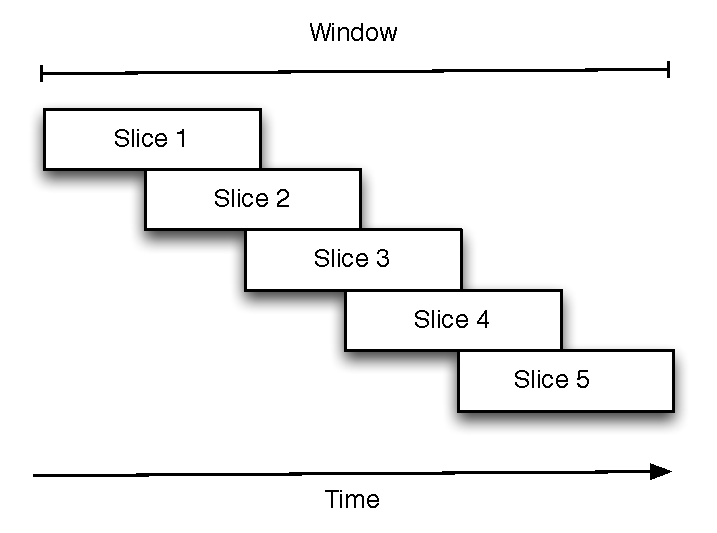
\includegraphics[width=2in]{./figures/slidingWindowSlices.pdf}
\caption{Sliding Window and Overlapping Slices}
\label{fig:windowSlices}
\end{center}
\end{figure}

From these features, we use AdaBoost to combine support vector machines (SVMs) and random forests (RFs) into an ensemble classifier to discriminate between bursty and non-bursty tokens.
To cast this task as a machine learning problem, however, we require positive and negative token samples on which our classifier can be trained.
While obtaining positive samples of bursty tokens is straightforward (we can at least use keywords from the baseline as well as event-specific tokens like names of scoring players or locations of events), determining negative samples is more difficult since it is hard to know all the events that may burst on Twitter at any moment.
Fortunately, we can circumvent this difficulty by automatically classifying all stop words as negative, non-bursty tokens, and Python's NLTK\footnote{http://www.nltk.org} library provides convenient lists of stop words for several languages.

It is important to note here that we perform this classification without any semantic or language-based filtering or normalization, and the only data we discard in this analysis are retweets and hashtags.

\subsubsection{Temporal Features}

While previous work already covers burst detection, only a subset is relevant to the streaming case presented herein, and we integrated those into our system.
Beyond these existing features, we also developed a number of features that should yield higher weights for tokens that deviate significantly from normal posting frequencies:

\begin{itemize}
\item \textbf{Frequency Regression} Given the log of a token's frequency at each slice in the current window, take the slope of the best-fitting line.
\item \textbf{Message Frequency Regression} Given the log of the number of tweets in which a token appears for each slice in the current window, take the slope of the best-fitting line.
\item \textbf{User Frequency Regression} Given the log of the number of users using a token at each slice in the current window, take the slope of the best-fitting line.
\item \textbf{Average Frequency Difference} The difference between the token's frequency in the most recent slice and the average frequency across the current window.
\item \textbf{Message Average Frequency Difference} The difference between the number of messages in which a token appears in the most recent slice and the average number of messages containing that token across the current window.
\item \textbf{User Average Frequency Difference} The difference between the number of users who use a token in the most recent slice and the average number of users across the current window.
\item \textbf{Inter-Arrival Time} The average number of seconds between token occurrences in the given window.
\item \textbf{Entropy} The entropy of the set of tweets containing a given token.
\item \textbf{TF-IDF} The term frequency, inverse document frequency for a each token.
\item \textbf{TF-PDF} A modified version of TF-IDF called term frequency, proportional document frequency \cite{Bun:2002:TEN:645962.674082}.
\item \textbf{BursT} Weight using a combination of a given token's actual frequency and expected token frequency \cite{Lee:2011:BDT:2009463.2009531}.
\end{itemize}

We also normalize each window's feature vectors into the range $[0, 1]$ to avoid biases from scale during classification by taking the maximum and minimum values for each feature in the current window.

\subsubsection{Training the Ensemble Classifier}

Discriminating between bursty tokens and stop words necessitated the use of a classification algorithm, and many different such algorithms exist.
In particular, the Scikit-learn Python package provides implementations for SVMs and RFs as well as an implementation of the ensemble classifier AdaBoost \cite{scikit-learn}.
Both SVMs and RFs have tunable parameters to select before integrating into AdaBoost, however, so we developed a grid search strategy to select parameters based on the F1 scores on our training and testing data.

For SVMs, we used the radial basis kernel, which has two parameters: cost $c$ and kernel coefficient $\gamma$.
In searching the space of $c$ and $\gamma$, the grid covered powers of two such that $c = 2^x$, $x \in [-2, 10]$ and $\gamma = 2^y$, $y \in [-2, 5]$.
For each pair of parameter values, we trained thirty different classifiers using repeated random subsampling, took the average F1 score, and selected the parameter set with the highest F1 score.
Selecting parameter values for RFs was similar for the number of estimators $n$ and feature count $c'$ such that $n = 2^x$, $x \in [0, 10]$ and $c' = 2^y$, $y \in [1, 11]$.
This training procedure yielded the results shown in Table \ref{tab:scores}.

\begin{table}[htdp]
\caption{Classifier Parameter Scores}
\begin{center}
\begin{tabular}{|c|c|c|c|c|}
\hline
\textbf{Classifier} & \textbf{Params} & \textbf{F1-Score} \\ \hline
SVM & $c=64,$ & 0.588410 \\ 
& $\gamma=4$ & \\ \hline
RF & trees = 128, & 0.575301 \\
& features = 9 &  \\ \hline
\end{tabular}
\end{center}
\label{tab:scores}
\end{table}

These two classifiers were then combined using the Scikit-learn's AdaBoost implementation with four estimators.
We then applied the resulting AdaBoost classifier to all the training data and expanded our set of known bursty tokens with those tokens that had a greater than 90\% likelihood of being part of the bursty class in one round of self-training (Scikit's AdaBoost implementation provides likelihoods for tokens it predicts).

Regarding sliding window and slice size, preliminary investigations seemed to illustrate a window size of ten minutes with a slice size of three minutes (each slice overlapped the next by two minutes) lead to acceptable results.

\section{Experimental Results}
\label{sect:results}

To restate, the research question posed in this work is to determine whether a language-agnostic, streaming event detection scheme can perform as well as a domain-specific frequency-based method in detecting events in sporting competitions.
We answer this question across three separate sporting events: the final two games of the 2013 MLB World Series, the 2014 NFL Super Bowl, and the final two matches of the 2014 FIFA World Cup.

For each event, we generated ROC curves by varying a threshold parameter and calculating the true and false positive rates.
In the baseline approach, our threshold parameter controlled the minimum difference between current frequency and average frequency over the sliding window.
For our LABurst method, the ROC curve was generated by varying the minimum number of tweets a window must contain for an event to be detected.
We then compared the area under the curve (AUC) metric to determine the difference in performance between the two methods.
Prior to presenting comprehensive results, we first present performance curves for each event type.

\subsection{2013 World Series}

For the 2013 World Series between the Boston Red Sox and the St. Louis Cardinals, we explored only the final two games on 28 October and 30 October of 2013.
These games contained fourteen events of interest: four game starts/ends and ten instances of points scored.
The two tested techniques exhibited similar performance, with a difference of only 0.02 (the baseline with 0.76 and the language-agnostic bursty method with 0.74).
Figure \ref{fig:roc2013WorldSeries} shows the how these two curves compare graphically, and we can see that neither curve completely dominates the other, and both perform better than random guessing.

\begin{figure}[hbtp]
\begin{center}
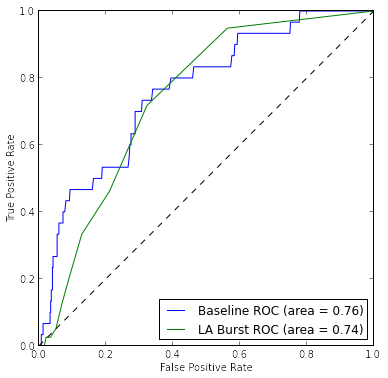
\includegraphics[width=2.5in]{./figures/roc_2013_WorldSeries.png}
\caption{ROC Curves for the 2013 World Series}
\label{fig:roc2013WorldSeries}
\end{center}
\end{figure}

\subsection{2014 Super Bowl}

Since the 2014 Super Bowl was a single-day competition, we covered the entire game between the Seatlle Seahawks and the Denver Broncos on 2 February 2014, which contained twelve events: a game start, an end, and ten instances of points scored.
The difference between the two mechanisms (shown in Figure \ref{fig:roc2014SuperBowl}) is more pronounced with a difference in AUC near 0.1, with the baseline performing better.
LABurst exhibited a much higher false-positive rate in comparison to the baseline, which may be explained later in \ref{sect:eventDiscovery}.

\begin{figure}[hbtp]
\begin{center}
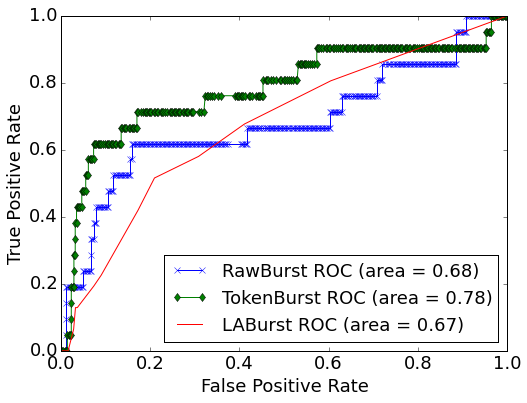
\includegraphics[width=2.5in]{./figures/roc_2014_SuperBowl.png}
\caption{ROC Curves for the 2014 Super Bowl}
\label{fig:roc2014SuperBowl}
\end{center}
\end{figure}

\subsection{2014 World Cup}

As with the World Series, our World Cup analysis covered the final two matches of tournament: the 12 July match between the Netherlands and Brazil for third place, and the final match on 13 July between Germany and Argentina for first place.
These matches contained the most events with a total of seventeen: four game starts/ends, nine penalty cards issued, and four goals scored.
Unlike the World Series and Super Bowl, however, the difference between the baseline and LABurst shows our LABurst method actually outperforms the baseline here with a difference in AUC of approximately 0.05.

\begin{figure}[hbtp]
\begin{center}
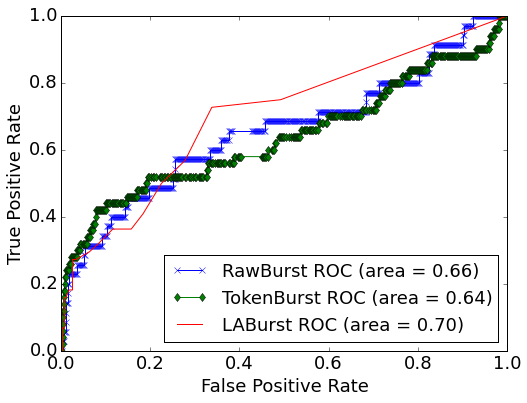
\includegraphics[width=2.5in]{./figures/roc_2014_WorldCup.png}
\caption{ROC Curves for the 2014 World Cup}
\label{fig:roc2014WorldCup}
\end{center}
\end{figure}

\subsection{Composite Results}

To compare comprehensive performance, we look to Figure \ref{fig:rocComprehensive}, which shows ROC curves for both methods across all three event types.
From this figure, we see the two methods perform nearly identically with AUC values of 0.7187 for the baseline and 0.7052 for our language-agnostic technique.
Assuming equal cost for false positives and false negatives and optimizing for the largest difference between true positive rate (TPR) and false positive rate (FPR), the baseline method shows 0.5581 and 0.1408 respectively with a difference of 0.4174 at a threshold value of 13.2.
Our language-agnostic method, on the other hand, has a TPR of 0.7105 and FPR of 0.3518 with a difference of 0.3587 at a threshold value of 2.
From these values, we see our approach achieves a higher true positive rate but at a cost of a higher false positive rate as a result.

\begin{figure*}[hbtp]
\begin{center}
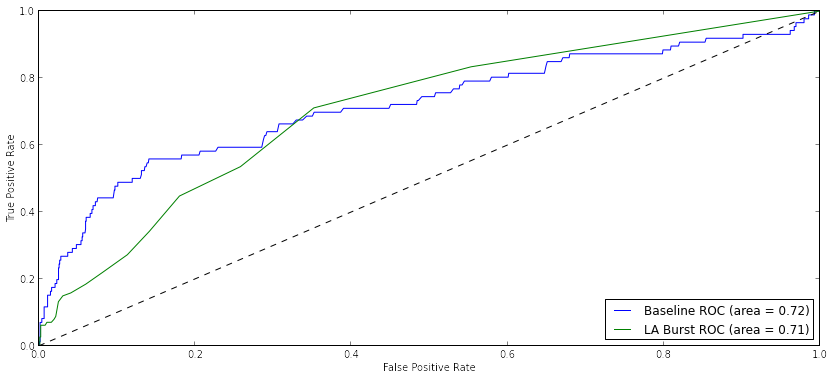
\includegraphics[width=5in]{./figures/roc_Comp.png}
\caption{Composite ROC Curves}
\label{fig:rocComprehensive}
\end{center}
\end{figure*}

\subsection{Earthquake Detection}

Detecting sub-events within sporting competitions as described above is a useful task for areas like advertising or automated highlight generation, but a more interesting and worthwhile task would be to detect higher-impact events like natural disasters.
The typical frequency-based approach is more difficult here as it is impossible to know what events are about to happen, and a list of target keywords to detect all such events would be long, leading to false positives.
Our method could be highly beneficial here as one would not need to know the target language or other pre-specified information.
Since Sakaki showed the feasibility of detecting earthquakes using Twitter, we pulled Twitter data for two earthquakes in Japan: a 7.1-magnitude quake off the coast of Honshu on 25 October 2013, and a 6.5-magnitude quake off the coast of Iwaki on 11 July 2014.

To determine whether our approach could detect these earthquake events, we applied the classifier trained and tested for the sporting domain to these Twitter sets and tracked the frequency of the term ``earthquake'' simultaneously.
Figures \ref{fig:2013Japan} and \ref{fig:2014Japan} show the frequencies for both methods for the 2013 and 2014 earthquakes respectively; the red dots indicate the earthquake times as reported by the United States Geological Survey (USGS).
From these figures, one can see the token ``earthquake'' sees a significant increase in usage when the earthquake occurs, and our language-agnostic method experiences a similar increase at the same moment for both events.
That is, both techniques identify the earthquake simultaneously.

\begin{figure}[hbt]
\begin{center}
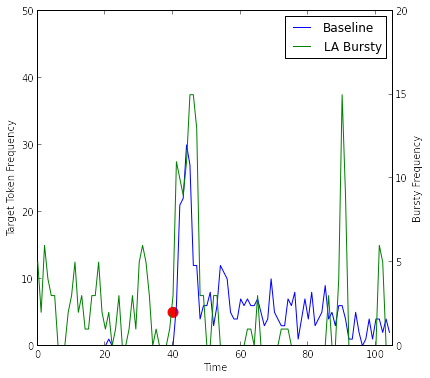
\includegraphics[width=2.5in]{./figures/2013-japan-quake.png}
\caption{Honshu, Japan Earthquake - 25 October 2013}
\label{fig:2013Japan}
\end{center}
\end{figure}

\begin{figure}[hbtp]
\begin{center}
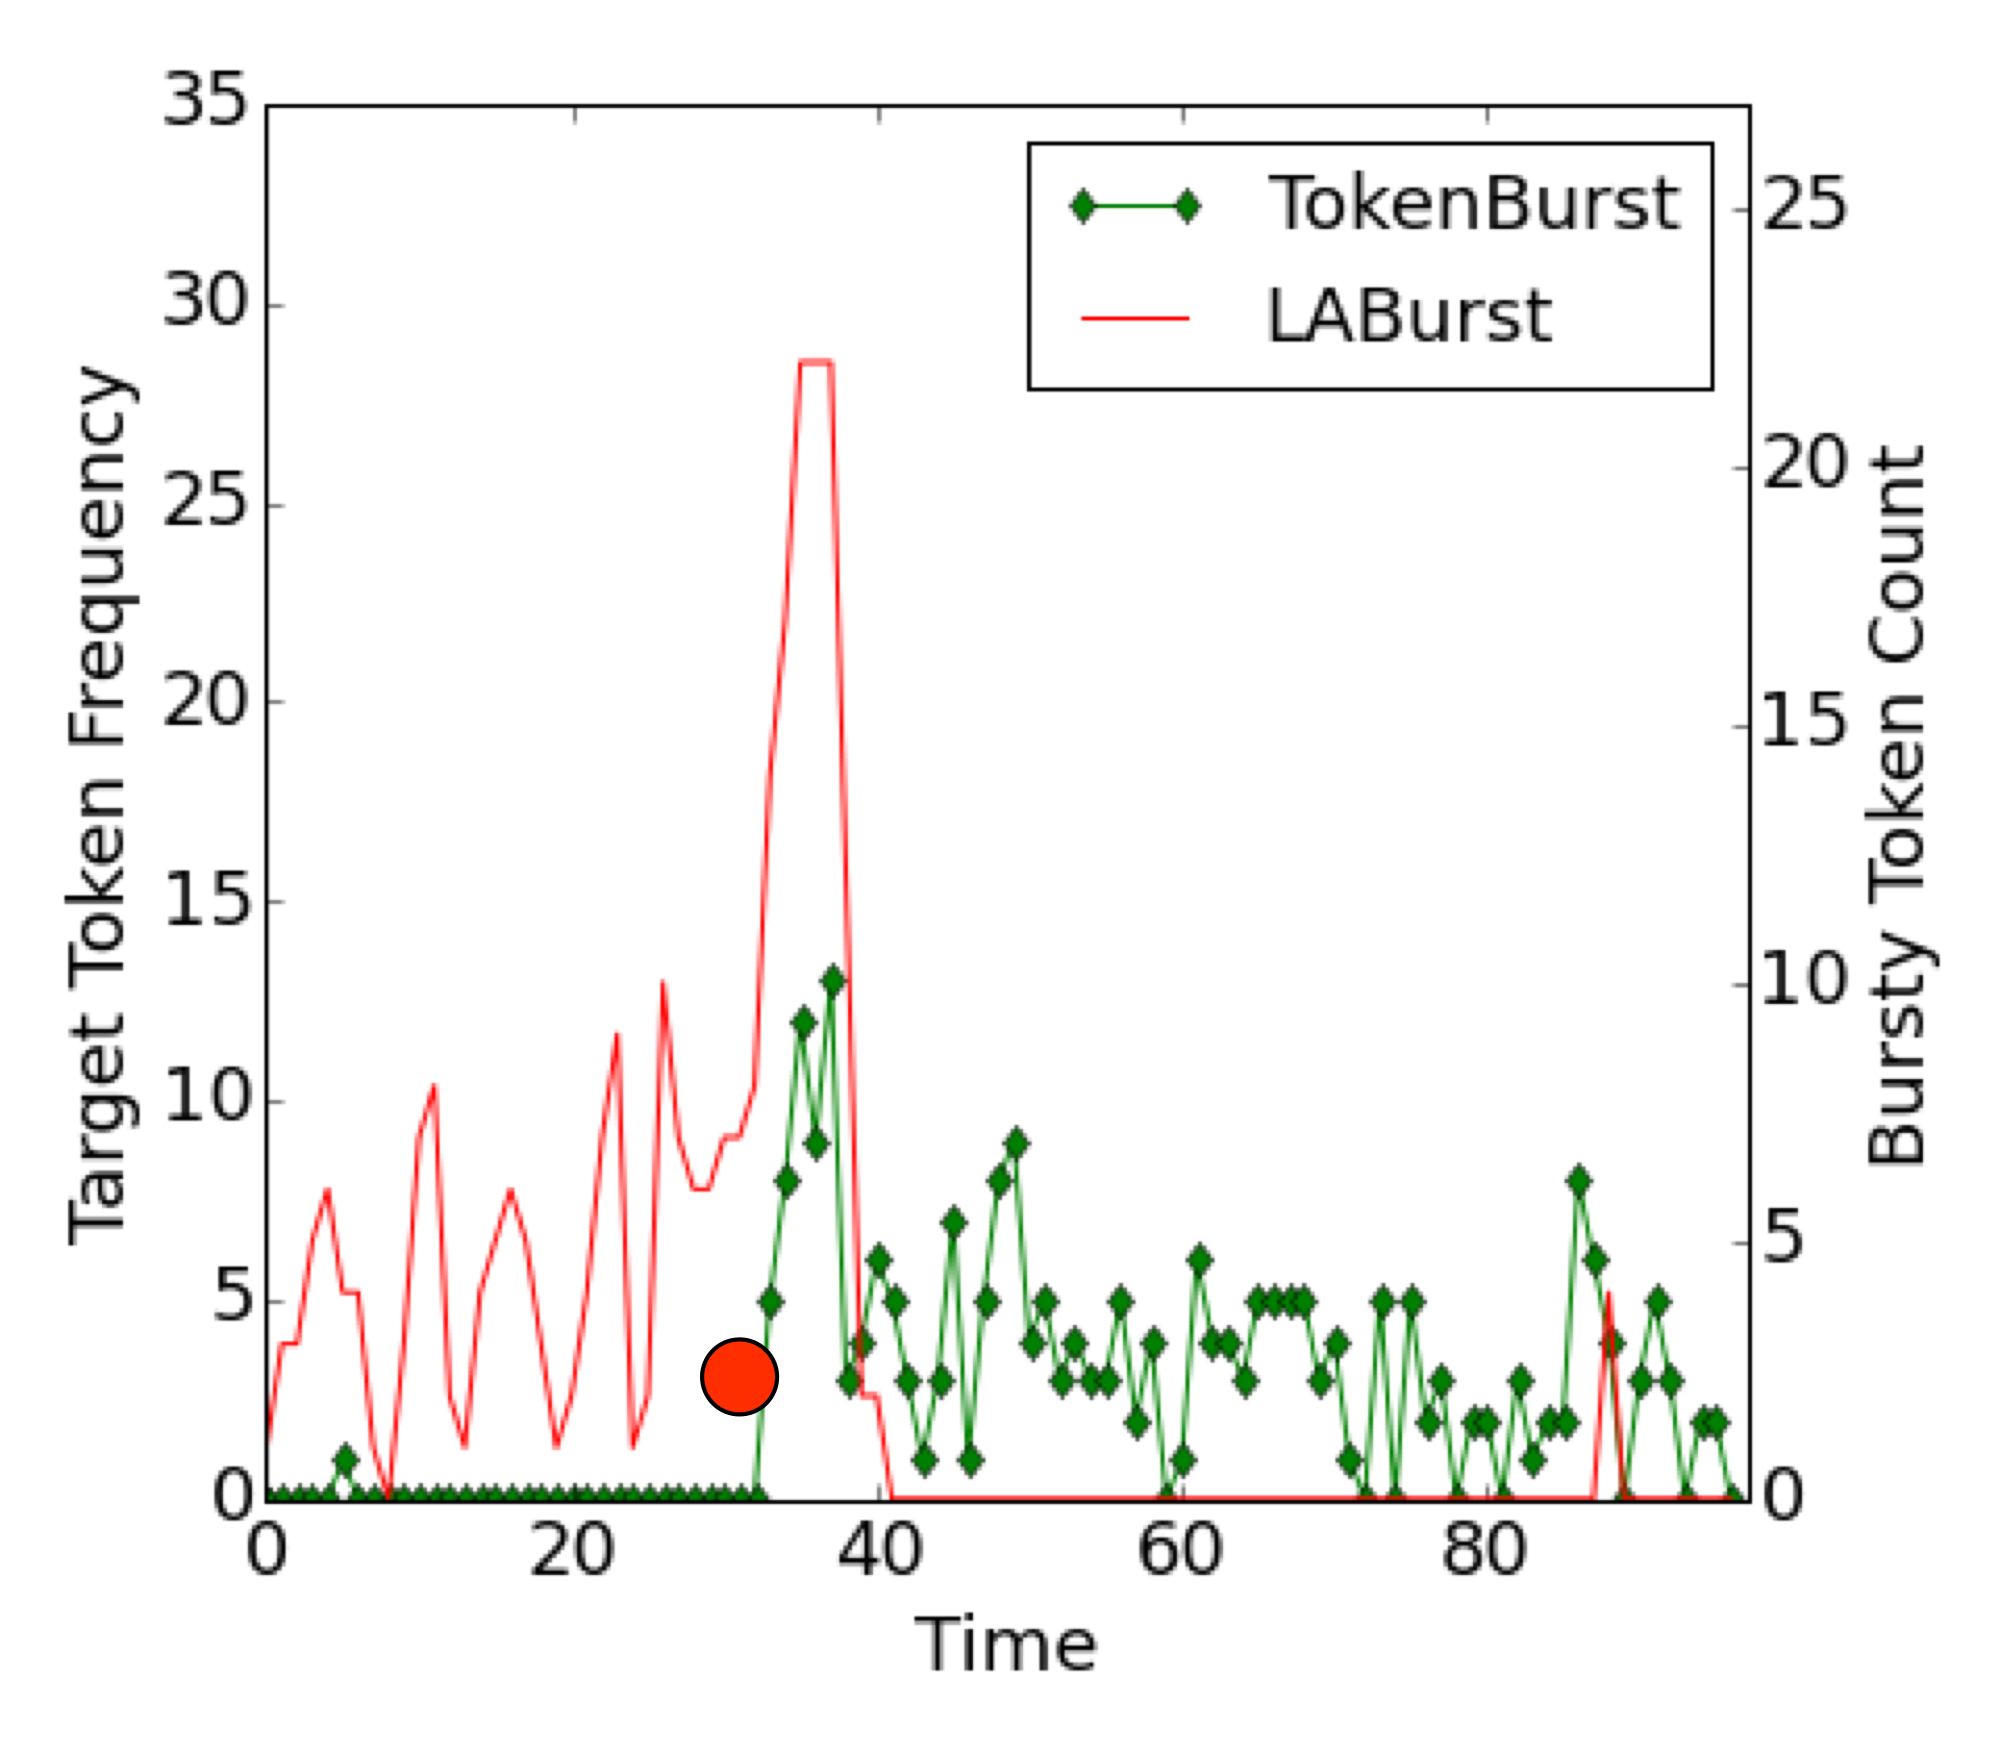
\includegraphics[width=2.5in]{./figures/2014-japan-quake.png}
\caption{Iwaki, Japan Earthquake - 11 July 2014}
\label{fig:2014Japan}
\end{center}
\end{figure}

Given our method's success here, one can now ask what tokens we identified as bursting when the earthquakes occurred.
Many of the tokens are in Japanese, and tokens at the peak of the earthquake events are shown in Table \ref{tab:japanTokens}.
We also extracted tweets from our data that contain the highest number of these tokens for the given time period, a selection of which include, \begin{CJK}{UTF8}{\myfont}``地震だあああああああああああああああああああああ,'' ``今回はチート使ってないから地震わからなかった,'' and ``地震だー.'' \end{CJK}
Google Translate\footnote{http://translate.google.com} translates these tweets as ``Ah ah ah ah ah ah ah ah ah Aa's earthquake,'' ``I did not know earthquake because not using cheat this time,'' and ``Over's earthquake'' respectively.

\begin{table}[htdp]
\caption{Tokens Classified as Busting During Events}
\begin{center}
\begin{tabular}{|p{1.45in} | p{1.45in} |}
\hline
\multicolumn{1}{|c|}{\textbf{Match}} & \multicolumn{1}{|c|}{\textbf{Bursty Tokens}} \\ \hline
Honshu, Japan -- 25 October 2013 & \c{c}dostum, \begin{CJK}{UTF8}{\myfont} 丈, 地, 夫, 怖, 波, 注, 津, 源, 福, 震 \end{CJK} \\ \hline
Iwaki, Japan -- 11 July 2014 & antojo, comida, sammy, \begin{CJK}{UTF8}{\myfont} び, ゆ, ビビ, 地, 怖, 急, 福, 警, 速, 震 \end{CJK} \\ \hline
\end{tabular}
\end{center}
\label{tab:japanTokens}
\end{table}

\section{Analysis}
\label{sect:analysis}

In comparing the baseline and language-agnostic techniques, it is important to understand the baseline provides little in the way of discovering previously unknown tokens or significant events that do not conform to a priori knowledge.
The real power of the language-agnostic method described herein addresses such deficiencies directly by identifying specific tokens that burst along with a significant event \emph{and} by capturing unexpected events.

\subsection{Identifying Event-Related Tokens}

As mentioned, where the baseline requires the user to specify interesting or event-related tokens prior to any data processing or analysis, our approach identifies these event-related tokens automatically.
These tokens may include misspellings, colloquialisms, and cross language boundaries, which makes them hard to know before hand.
The 2014 World Cup presents an interesting case for finding these otherwise unexpected tokens because the event has enormous international viewership; as such, many Twitter users of many different languages are likely tweeting about the same event.

To explore the tokens generated during these high-profile events, we look to those tokens identified as bursting during several events in the final two World Cup matches.
Table \ref{tab:burstyTokens} shows a selection of events from these matches and a subset of those tokens classified as bursting during the events (one should note the list is not exhaustive owing to formatting and space constraints).

\begin{table}[htdp]
\caption{Tokens Classified as Busting During Events}
\begin{center}
\begin{tabular}{|p{0.75in}|p{0.7in}| p{1.45in} |}
\hline
\multicolumn{1}{|c|}{\textbf{Match}} & \multicolumn{1}{|c|}{\textbf{Event}} & \multicolumn{1}{|c|}{\textbf{Bursty Tokens}} \\ \hline
Brazil v. Netherlands, 12 July 2014 & Netherlands' Van Persie scores a goal on a penalty at 3', 1-0 & 0-1, 1-0, 1:0, 1x0, card, goaaaaaaal, goal, gol, goool, holandaaaa, k\i{}rm\i{}z\i{}, pen, penal, penalti, p\^{e}nalti, persie, red \\ \hline
Brazil v. Netherlands, 12 July 2014 & Brazil's Oscar get's a yellow card at 68' & dive, juiz, penalty, ref \\ \hline
Germany v. Argentina, 13 July 2014 & Germany's G\"{o}tze scores a goal at 113', 1-0 & goaaaaallllllll, goalllll, godammit, goetze, gollllll, gooooool, gotze, gotzeeee, g\"{o}tze, nooo, yessss, \begin{CJK}{UTF8}{\myfont} ドイツ\end{CJK} \\ \hline
\end{tabular}
\end{center}
\label{tab:burstyTokens}
\end{table}

Several interesting artifacts emerge from this table, first of which is that one can get an immediate sense of the detected event from tokens our algorithm presents. 
For instance, the prevalence of the token ``goal'' and its variations clearly indicate a team scored in the first and third events in Table \ref{tab:burstyTokens}; similarly, bursting tokens associated with the middle event regarding Oscar's yellow card reflect his penalty for diving.
Beyond the pseudo event description put forth by the identified tokens, this reference to diving and to specific player and teams names in the first and third events are also of significant interest.
In the first event, one can infer that the Netherlands scored since ``holandaaaa'' is flagged along with ``persie'' from the Netherlands' player Van Persie, and likewise for Germany's G\"{o}tze in the third event (and the accompanying variations of his name).
These terms would be difficult to capture beforehand as would be required in the baseline and would likely not be related to every event or every type of sporting event.

Finally, the last artifact of note is that the set of bursty tokens displayed includes tokens from several different languages: English for ``goal'' and ``penalty,'' Spanish for ``gol'' and ``penal,'' Brazilian Portuguese for ``juiz'' (meaning ``referee''), as well as the Arabic for ``goal'' and Japanese for ``Germany.''
Since these words are semantically similar but syntactically dissimilar, typical normalization schemes could not capture these connections.
Instead, capturing these words in the baseline would require a pre-specific keyword list in all possible languages or the inclusion of an expensive machine translation system that was also capable of normalizing within different languages (to collapse ``goool'' down to ``gol'' for example).

\subsection{Undocumented Event Discovery}
\label{sect:eventDiscovery}

One particular weakness present in the baseline is that it is unable to capture unexpected events or events that do not conform to the keyword list.
This deficiency means analysts might miss significant events within these competitions, especially if they are not directly related to scores or penalties, such as Uruguay's Luis Suarez's biting the Italy's Giorgio Chiellini during a World Cup match on 24 June since no foul was called at the time.
Other instances of particularly dramatic play or events that happen at the larger sporting event but not necessarily on the field might be missed as well.

We can see instances of such omissions in the last game of World Cup.
Figure \ref{fig:worldCupFreqs} shows the frequencies for target tokens for the baseline in blue and bursty tokens for our method in green.
From this graph, we can see the first, obvious incidence in Peak \#1 where our bursty method exhibits a peak that is missed by the baseline in the first few points of data.
The primary tokens appearing in this peak are ``puyol,'' ``gisele,'' and ``bundchen,'' which correspond to former Spanish player Carles Puyol and model Gisele Bundchen, who presented the World Cup trophy prior to the match.
Peak \#2, slightly more than eighty minutes into the data (which is sixty minutes into the match), our burst analysis sees another peak that is otherwise relatively minor in the baseline graph.
Upon further exploration, tokens present in this peak refer to Argentina's substituting in Ag\"{u}ero for Lavezzi at the beginning of the match's second half.

\begin{figure}[hbtp]
\begin{center}
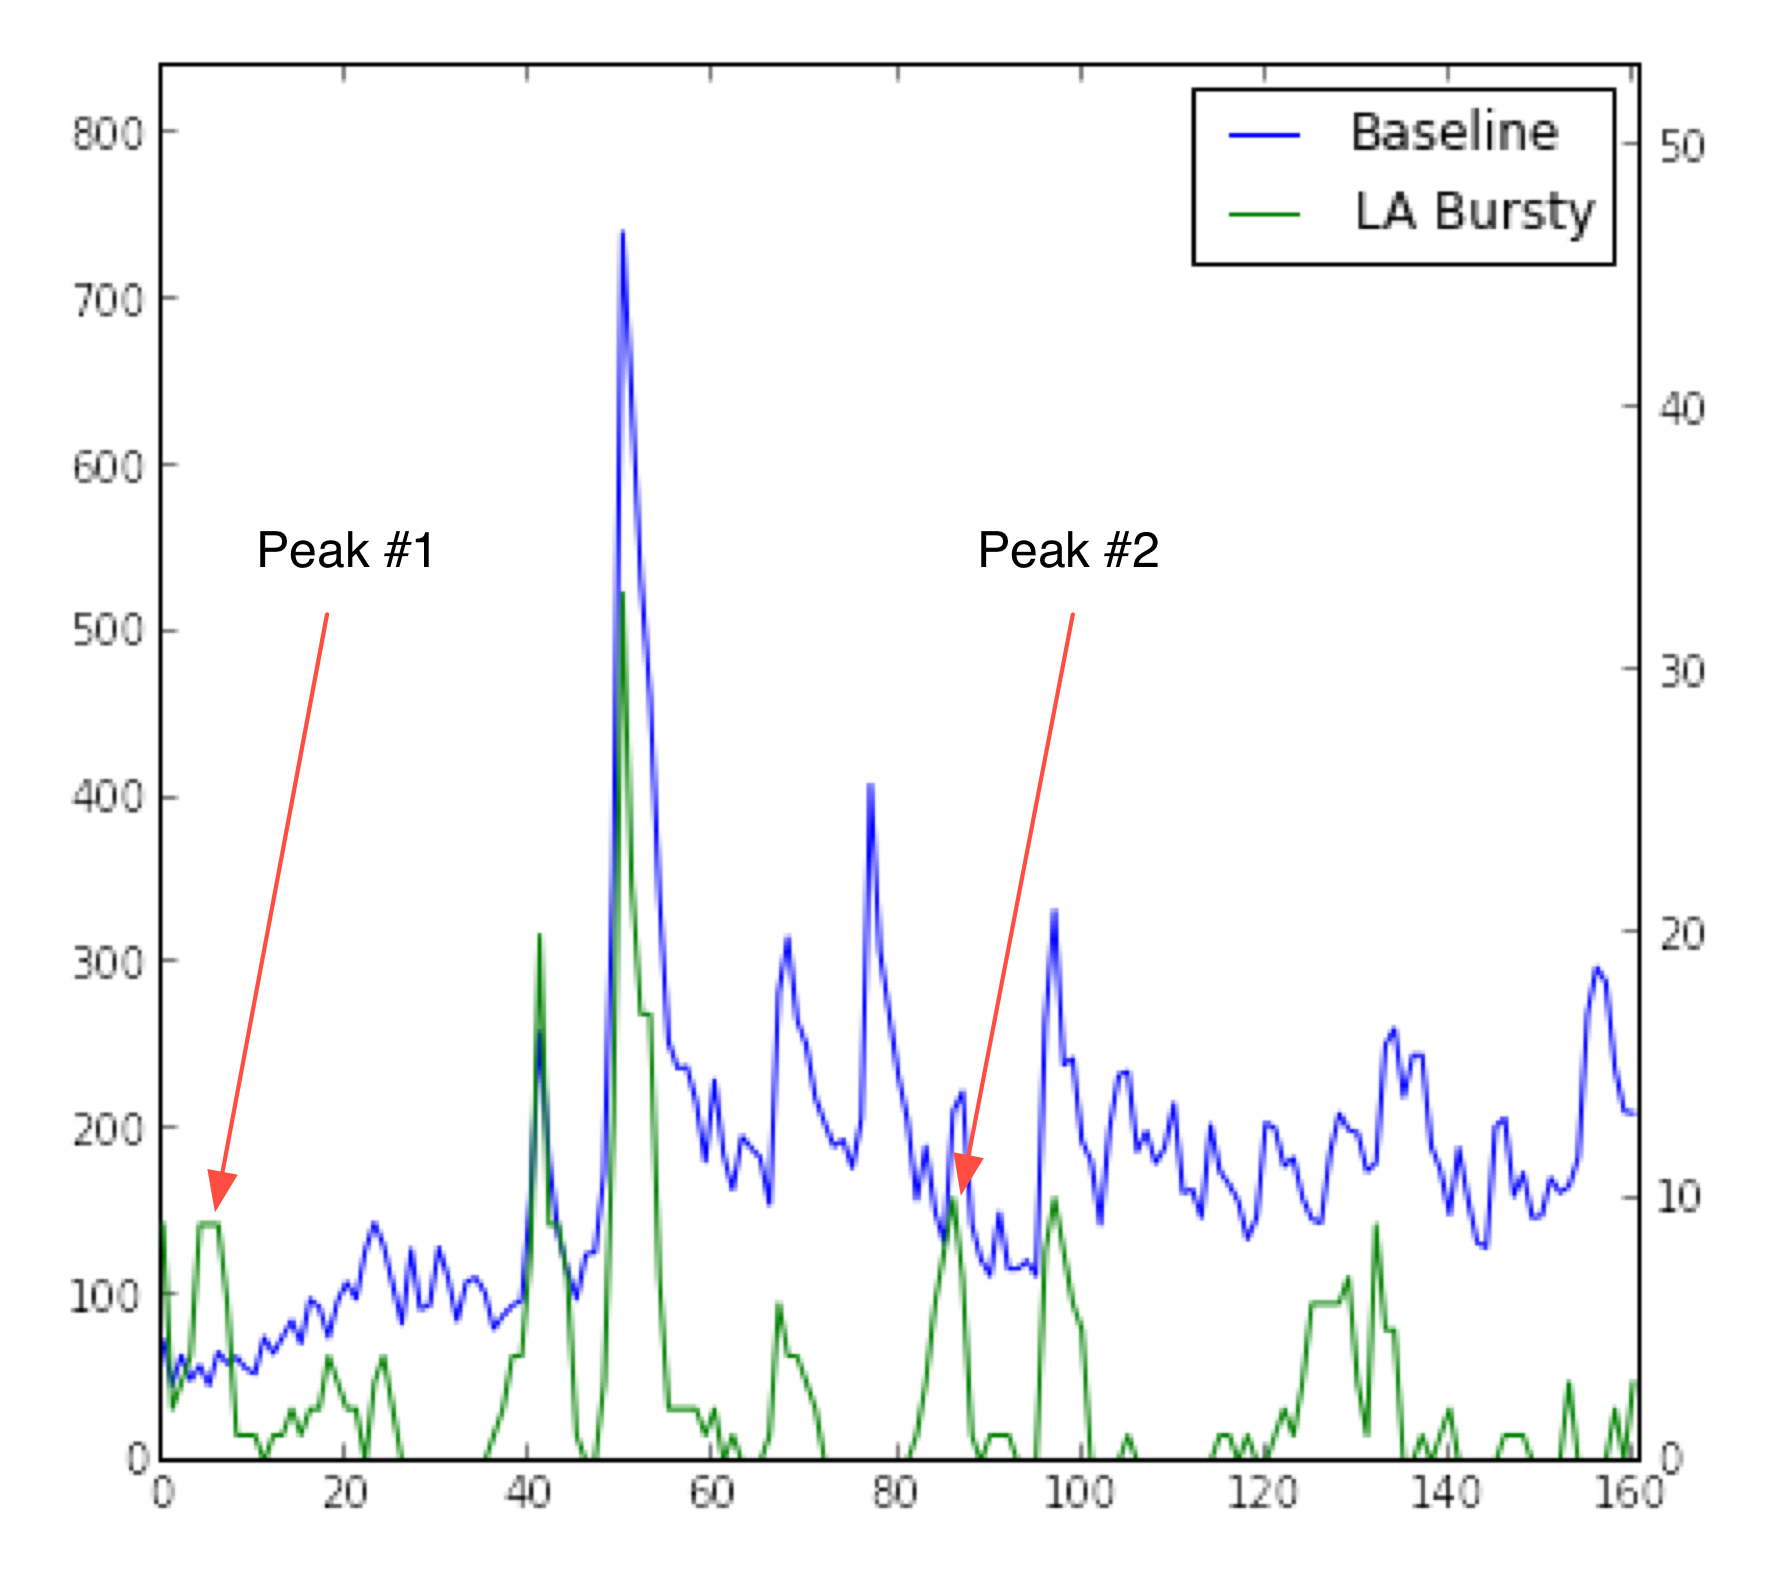
\includegraphics[width=3.25in]{./figures/wc0713freq-labeled.png}
\caption{Baseline and LA Bursty Frequencies}
\label{fig:worldCupFreqs}
\end{center}
\end{figure}

Given our detection of these additional non-score-/non-penalty-related events, it is perhaps unsurprising that our burst detection technique exhibits a higher false-positive rate compared to the baseline.
Since our approach is both language- and domain-agnostic, it makes sense that it would detect additional events beyond the game start/end, score, and penalty events our data counts as ground truth.
A better comparison between the accuracies of the two approaches may be to identify only those peaks in which the keywords used in the baseline are identified as bursty in our method, but such a test disregards our approach's additional power.

\subsection{Real-Time Usage and Event Persistence}

In comparing these two event detection methods, we must also address their abilities to handle streaming data and the lag between an event and its detection by either of these mechanisms.
The baseline technique processes data minute by minute and therefore has at most a minute of lag between input and discovery.
Our technique, on the other hand, exhibits a lag equal to the slice size, which in the case of this paper is three minutes.

Another important aspect to consider is the length of time in which an event's peak persists.
For the baseline, event detection achieves its highest accuracy when events are flagged in the minute they occur and the minute immediately following.
Our approach logically follows the slice length such that events persist for three minutes.

\section{Future Work}
\label{sect:future}

% Real streaming context, Different classifiers, different levels of granularity, more domain adaptation research, temporal topic clustering, Facebook?
While the experiments outlined herein establish the utility of language-agnostic event detection, several avenues of research can follow up on this foundation.
First, though this work is applied in the streaming context, little effort was made to enforce near-real-time computation constraints; with the growing popularity of stream-centric processing frameworks like Apache Storm (as used by Petrovi\'{c} et al.) or Apache Spark Streaming, one has considerable latitude in exploring ways to enforce such constraints.
Secondly, our selection of classifiers used in our ensemble was based primarily on ease of use given our features; deep learning systems are more complex but could provide enhanced capabilities in detecting bursting patterns in social media streams.
Thirdly, we specifically targeted short-term, instantaneous events, but it is possible that these same techniques could be applied at different levels of granularity (per hour or per day for instance) to detect events of larger scales; one could then apply Kleinberg's notion of event hierarchies across multiple temporal granularities and track different aspects of the same event.
Additionally, an implicit assumption made in this work is that tokens that experience bursts at the same time are related in some way, which allows us to detect events using token frequency; this assumption has interesting consequences with regarding to language-agnostic topic detection.
That is, one could cluster tokens with similar temporal signatures to identify topics across languages, which would otherwise be impossible if one were to rely solely on semantic similarity or would require applying machine translation to reduce all text in the stream to the same language.
Finally, though this paper exclusively leverages data from Twitter's public stream, our techniques should be applicable to streams from other social networks as well, and how events burst on more media-centered networks like Flickr or Pinterest might reveal interesting photographic representations of an event.

\section{Conclusions}
\label{sect:conlusions}

To revisit our motivations, the goal for this experiment was to demonstrate the feasibility of detecting events and event-related tokens through analyzing temporal characteristics from unfiltered Twitter data streams.
While many social media-based event detection systems require some form of query-based filtering and language model processing, our approach is more flexible, lighter weight, and easily adaptable to different domains.
Our results show that by leveraging temporal characteristics to identify bursty tokens and using frequency of these bursty tokens, we can detect significant events across a collection of disparate sporting competitions with a level of performance nearly equivalent to an existing, domain-specific baseline.

Similar performance to the baseline is only part of the story, however, as our approach offers notable flexibility in identifying bursting tokens without normalization and across language boundaries.
With this versatility also comes support for event description since we no longer rely on predetermined keywords; that is, we can get a sense of the occurring event by inspecting the bursty tokens.
Finally, these advantages culminate in powerful tool for event \emph{discovery} in that it can detect events we did not expect to occur, regardless of the source language, which makes this technique particularly useful for journalists and newswire sources who have a need to know about events on the ground, as they happen but cannot know a priori what the event may be about in all cases.

%\end{document}  % This is where a 'short' article might terminate

%ACKNOWLEDGMENTS are optional
\section{Acknowledgments}
This work made use of the Open Science Data Cloud (OSDC), which is an Open Cloud Consortium (OCC)-sponsored project. 
The OSDC is supported in part by grants from Gordon and Betty Moore Foundation and the National Science Foundation and major contributions from OCC members like the University of Chicago. 

%
% The following two commands are all you need in the
% initial runs of your .tex file to
% produce the bibliography for the citations in your paper.
\bibliographystyle{abbrv}
\bibliography{sources}  % sigproc.bib is the name of the Bibliography in this case
% You must have a proper ".bib" file
%  and remember to run:
% latex bibtex latex latex
% to resolve all references
%
% ACM needs 'a single self-contained file'!
%
%APPENDICES are optional
%\balancecolumns
\end{document}
